% \begin{tikzpicture}[scale=1.2]

% % Draw the global square domain
% \draw[thick] (0,0) rectangle (3,3);
% % \node at (3.3,3.3) {$\Omega$};

% % Draw vertical and horizontal grid lines
% \foreach \x in {1,2} {
%     \draw[thick] (\x,0) -- (\x,3);
%     \draw[thick] (0,\x) -- (3,\x);
% }

% % Label subdomains
% \foreach \i in {0,1,2} {
%     \foreach \j in {0,1,2} {
%         \pgfmathtruncatemacro{\idx}{\i*3 + \j + 1}
%         \node at (0.5 + \j, 2.5 - \i) {$\Omega_{\idx}$};
%     }
% }

% \end{tikzpicture}
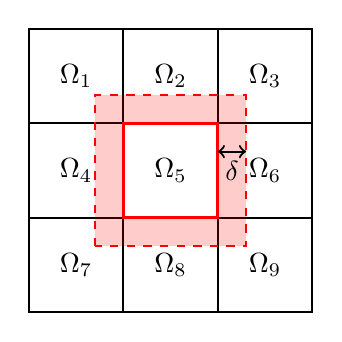
\begin{tikzpicture}[scale=1.2]

    % Draw the global square domain
    \draw[thick] (0,0) rectangle (3,3);
    
    % Draw vertical and horizontal grid lines
    \foreach \x in {1,2} {
        \draw[thick] (\x,0) -- (\x,3);
        \draw[thick] (0,\x) -- (3,\x);
    }
    
    % Label subdomains
    \foreach \i in {0,1,2} {
        \foreach \j in {0,1,2} {
            \pgfmathtruncatemacro{\idx}{\i*3 + \j + 1}
            \node at (0.5 + \j, 2.5 - \i) {$\Omega_{\idx}$};
        }
    }
    
    % Fill overlapping region around Omega_5
    \begin{scope}
        \clip (0.7,0.7) rectangle (2.3,2.3);
        \fill[red, opacity=0.2] (0.7,0.7) rectangle (2.3,2.3);
        \fill[white] (1,1) rectangle (2,2);
    \end{scope}
    
    % Redraw Omega_5 label on top
    \node at (1.5,1.5) {$\Omega_{5}$};

    % Draw dashed border for total overlap area
    \draw[dashed, thick, red] (0.7,0.7) rectangle (2.3,2.3);
    
    % Draw original Omega_5 boundary
    \draw[very thick, red] (1,1) rectangle (2,2);
    
    % Label delta
    \draw[<->, thick] (2,1.7) -- (2.3,1.7);
    \node[below] at (2.15,1.7) {$\delta$};
    
\end{tikzpicture}
    